Verifying LTSs against a modal $\mu$-calculus formula can be done by solving a parity game. This is done by translating an LTS in combination with a formula to a parity game, the solution of the parity game provides the information needed to conclude if the model satisfies the formula. This relation is depicted in figure \ref{fig:ltsverificationusingpg}. This technique is well known and well studied, in this section we will first look at parity games, the translation from LTS and formula to a parity game and finally what we can do with this technique to verify FTS.
\begin{figure}[h]
	\centering
	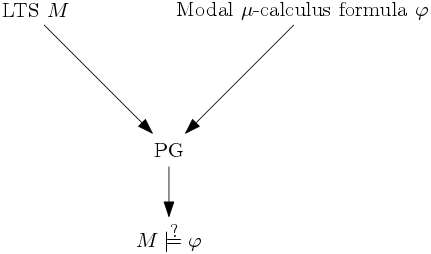
\includegraphics[scale=0.5]{Diagrams/LTSVerificationUsingPG}
	\caption[LTS verification using PG]{LTS verification using PG}
	\label{fig:ltsverificationusingpg}
\end{figure}

\subsection{Parity games}
\begin{definition}
	\label{def_PG}\cite{Bradfield2018}
	A parity game (PG) is a tuple $(V, V_0, V_1, E, \rho)$, where:
	\begin{itemize}
		\item $V = V_0 \cup V_1$ and $V_0 \cap V_1 = \emptyset$,
		\item $V_0$ is the set of vertices owned by player $0$,
		\item $V_1$ is the set of vertices owned by player $1$, 
		\item $E \subseteq V \times V$ is the edge relation,
		\item $\rho :  V \rightarrow \mathbb{N}$ is a priority assignment.
	\end{itemize}
\end{definition}
We write $\alpha \in \{0,1\}$ to denote an arbitrary player. We write $\overline{\alpha}$ to denote $\alpha$'s opponent, ie. $\overline{0} = 1$ and $\overline{1} = 0$.

A parity game is played by players 0 and 1. A play starts with placing a token on vertex $v \in V$. Player $\alpha$ moves the token if the token is on a vertex owned by $\alpha$, ie. $v \in V_\alpha$. The token can be moved to $w \in V$, with $(v,w) \in E$. A series of moves results in a sequence of vertices, called path. For path $\pi$ we write $\pi_i$ to denote the $i^{\text{th}}$ vertex in path $\pi$. A play ends when the token is on vertex $v \in V_\alpha$ and $\alpha$ can't move the token anywhere, in this case player $\overline{\alpha}$ wins the play. If the play results in an infinite path $\pi$ then we determine the highest priority that occurs infinitely often in this path, formally
\[ \max\{ p \ |\ \forall_j \exists_i j < i \wedge p = \rho(\pi_i) \}\] 
If the highest priority is odd then player $1$ wins, if it is even player $0$ wins.
\begin{figure}[h]
	\centering
	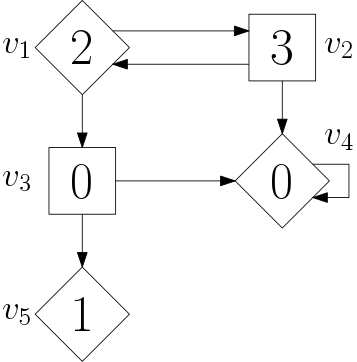
\includegraphics[scale=0.3]{Examples/SimplePG/PG}
	\caption[Parity game example]{Parity game example}
	\label{fig:simplepgpg}
\end{figure}

Figure \ref{fig:simplepgpg} shows an example of a parity game. We usually depict the vertices owned by player $0$ by diamonds and vertices owned by player $1$ by boxes, the priority is depicted inside the vertices. If the game starts by placing a token on $v_1$ we can consider the following exemplary paths:
\begin{itemize}
	\item $\pi = v_1v_3v_5$ is won by player $1$ since player $0$ can't move at $v_5$.
	\item $\pi = (v_1v_2)^\omega$ is won by player $1$ since the highest priority occurring infinitely often is 3.
	\item $\pi = v_1v_3(v_4)^\omega$ is won by player $0$ since the highest priority occurring infinitely often is $0$.
\end{itemize}


A strategy for player $\alpha$ is a function $\sigma : V^*V_\alpha \rightarrow V$ that maps a path ending in a vertex owned by player $\alpha$ to the next vertex. Parity games are positionally determined \cite{Bradfield2018}, therefore a strategy $\sigma: V_\alpha \rightarrow V$ that maps the current vertex to the next vertex is sufficient. 

A strategy $\sigma$ for player $\alpha$ is winning from vertex $v$ if and only if any play that results from following $\sigma$ results in a win for player $\alpha$. The graph can be divided in two partitions $W_0 \subseteq V$ and $W_1 \subseteq V$, called winning sets. If and only if $v \in W_\alpha$ then player $\alpha$ has a winnings strategy from $v$. Every vertex in the graph is either in $W_0$ or $W_1$ \cite{Bradfield2018}. Furthermore finite parity games are decidable \cite{Bradfield2018}.
\subsection{Creating parity games}

\subsection{FTSs and parity games}